% ### by András Kiss ###
% ### 2018.06.20 #######
% ### Homburg ##########
\documentclass[a4paper, 11pt]{article}
\usepackage{ae,aecompl}
\usepackage[T1]{fontenc}
\usepackage[utf8]{inputenc}
\usepackage{indentfirst}
\usepackage{xymtex}
\usepackage{multirow}
\usepackage{gensymb}
\usepackage{upgreek}
\usepackage[geometry]{ifsym}
\usepackage{subfig}
\usepackage[version=3]{mhchem}
\usepackage{float}
\usepackage{textcomp}
\frenchspacing
\usepackage[dvips]{graphicx}
\usepackage{color}
\usepackage{anysize}
\marginsize{3.2cm}{2.8cm}{3cm}{2cm}
\usepackage{enumerate}
\usepackage{cite}
\usepackage{listings}
\usepackage{setspace}
\usepackage{marginnote}
\setstretch{1.2}
\usepackage{xcolor}
\usepackage{listings}


\definecolor{codegreen}{rgb}{0,0.6,0}
\definecolor{codegray}{rgb}{0.5,0.5,0.5}
\definecolor{codepurple}{rgb}{0.58,0,0.82}
\definecolor{backcolour}{rgb}{0.95,0.95,0.92}
 
\lstdefinestyle{mystyle}{
    backgroundcolor=\color{backcolour},   
    commentstyle=\color{codegreen},
    keywordstyle=\color{magenta},
    numberstyle=\tiny\color{codegray},
    stringstyle=\color{codepurple},
    basicstyle=\footnotesize,
    breakatwhitespace=false,         
    breaklines=true,                 
    captionpos=b,                    
    keepspaces=true,                 
    numbers=left,                    
    numbersep=5pt,                  
    showspaces=false,                
    showstringspaces=false,
    showtabs=false,                  
    tabsize=2
}
 
\lstset{style=mystyle}

\begin{document}
\title{Deconvolution of amperometric SECM images recorded with the HEKA ElProScan}
\author{András Kiss, PhD}
\maketitle

This guide shows how to do the deconvolution of the .asc datasets produced with the HEKA SECM by Monika and Phillip in 2014. The example image \ref{fig:original11} shows the oxidation current at a 10 microemeter Pt disk electrode oxidizing H$_2$O$_2$. The current is decreased in the vicinity of the cell.

\begin{figure}
\centering
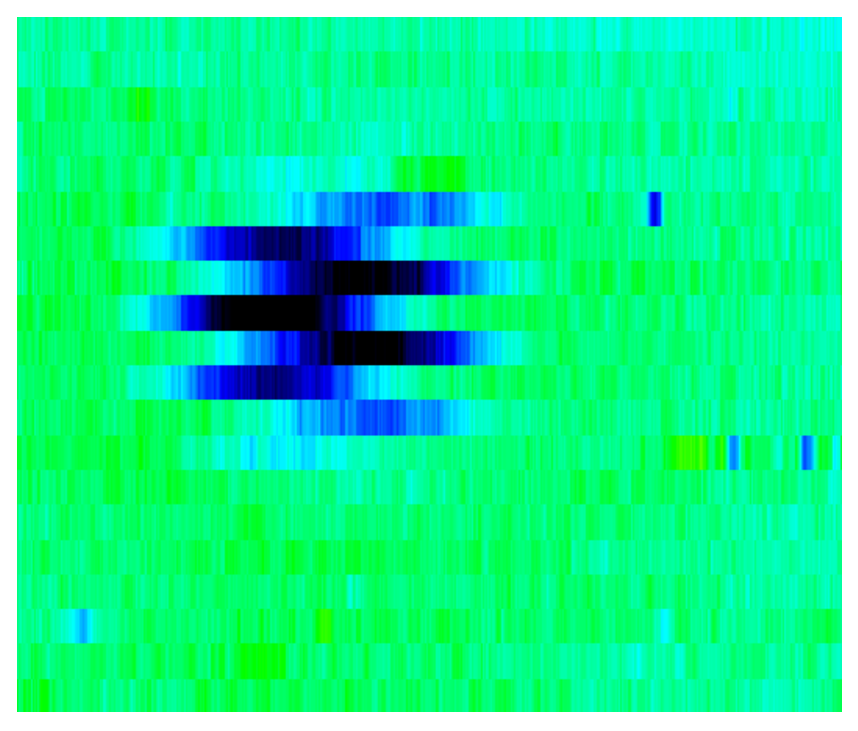
\includegraphics[width=0.5\textwidth]{original11.eps}
\label{fig:original11}
\caption{Original data recorded by Monika and Phillip. Image of a monocyte. Tip was d=10 $\upmu$m Pt, tip potential was 650 mV oxidizing H$_2$O$_2$. The image shows directional blur.}
\end{figure}


\begin{enumerate}
\item Multiplying X-ccordinate and current to get micrometer and picoampere.
   
\begin{lstlisting}[language=bash]
   awk '{$1, print $2*1000000, $3*1000000000000}' &&
   140128_1E1_11_3D.asc > 140128_1E1_11_3D_.asc
\end{lstlisting}

   This is a linux bash tool, of course it can be done with Origin or Excel.

\item Correct chronology of the measurement, by mirroring every other scanline. A script would be nice that does everything. I'm planning to write one using awk and sed. These are pretty good and efficient tools in Linux bash. Original data is in a format like this:

\begin{verbatim}
	scanline 1:
0
	2
	4
	...
	50

	scanline 2:
	0
	2
	4
	...
	50
\end{verbatim}

   But this is not the chronological order for the meander. The second scanline starts with the X-ccordinate 50! Correct order of the dataset:

\begin{verbatim}
        scanline 1:
        0
        2
        4
        ...
        50

        scanline 2:
        50
        48
        46
        ...
        0
\end{verbatim}

\item After I've done this, the data was ready for deconvolution, for which I've wrote the following FORTRAN program:

\begin{lstlisting}[language=fortran]
program deconvolution
implicit none

integer :: stat
real i, j, rc, e0, conv

rc=0.985

open(1,file='11.txt')
open(2,file='11_deconvoluted.txt')
read(1, *) i, j, e0
do
   read(1, *, iostat=stat) i, j, conv
   if (stat /= 0) exit
   write(2, *) i, j, ((conv - e0*rc)/(1-rc))
   e0=conv
end do
close(1) 
close(2)

end program deconvolution
\end{lstlisting}

I compiled the code with gfortran. Then I ran the resulting a.out (default output) as:

./a.out

I think even Excel can be used for deconvolution. The criteria is that the program should be able to do relative references.

\item To plot the original and the result, I've used gnuplot. Of course you can use Origin or other similar program.

\begin{lstlisting}{language=gnuplot}
set size ratio 0.8
set pm3d map
set dgrid3d 51, 40 , 10, gauss 1,1
set cntrparam levels auto 10
set term postscript enhanced color
set xlabel "X / {/Symbol m}m"
set ylabel "Y / {/Symbol m}m"
set palette rgbformulae 22, 13, -31 # quickgrid
set xtics font "Helvetica, 25"
set ytics font "Helvetica, 25"
set xlabel font ",25"
set ylabel font ",25"
set cblabel font ",25"
set cbtics font ",25"
set cblabel offset 4,0
set ylabel offset -3,0
set xlabel offset 0,-1
set xtics 0, 25, 50
set ytics 0, 19, 38
set yrange [0:38]
set xrange [0:50]
set cblabel "i / pA"
set cbrange [1.2:1.7]

set label "140128-1-E1-11-3D.asc" &&
	at 1, 35 tc rgb "white" font ",40" front
set out "11.eps"
splot "11.txt" u ($1):($2):($3) notitle
unset label

set label "140128-1-E1-11-3D.asc" && 
	at 1, 35 tc rgb "white" font ",40" front
set label "deconvoluted" &&
	at 1, 31 tc rgb "white" font ",40" front
set out "11_deconvoluted.eps"
splot "11_deconvoluted.txt" u ($1):($2):($3) notitle
unset label
\end{lstlisting}

Of course, gaussian filter is necessary to eliminate the unavoidable increase in noise after deconvolution. The line that does it is:

\begin{lstlisting}{language=gnuplot}
set dgrid3d 51, 40 , 10, gauss 1,1
\end{lstlisting}

\end{enumerate}

The results can be seen in Fig. \ref{fig:results}. This is the complete procedure to produce the figures from the raw data Phillip sent me.

\begin{figure}
\centering
\includegraphics[width=0.5\textwidth, angle=-90]{11.eps}
\includegraphics[width=0.5\textwidth, angle=-90]{11_deconvoluted.eps}

\label{fig:results}
\caption{Raw and deconvoluted images.}
\end{figure}



\end{document}

